The primary aim of this research is to enable us to collect a series of probe
requests and process them into a usable pedestrian footfall count. We do this by
using a Wi-Fi receiver to collect probe requests broadcast by mobile devices,
filtering out the background noise and aggregating them based on the device that
generated them. In this section, we begin by looking at the characteristics of
probe requests in detail, device a methodology to collect these probe requests
in public areas, examine the systemic biases and uncertainties in the data
collection method and device data processing methods to overcome these
challenges. Finally we compare the processed footfall counts to the ground truth
recorded by primary surveys.

Probe requests are a special type of management packets broadcast by Wi-Fi
enabled devices as part of the various functions such as scanning for available
APs, quick geolocation by triangulation based known APs, etc. These are
broadcast by all Wi-Fi enabled devices regardless of the manufacturer, type or
model of the devices though there is some variation on the frequency and the
information transmitted through them. In some cases, such as Android devices,
these are broadcast even when the Wi-Fi functionality has been turned off by
the user so that device can immediately connet to networks when the
functionality is switched back on. Since some devices even use the probe
requests as a less accurate form of localisation they keep sending probe
requests as well. Thus these signals can be used to reliably identify the
presence of Wi-Fi enabled mobile devices. Being a first step of connection
initiated by the mobile device, these packets have information regarding the
characteristics of the mobile device itself. Some of the key information we can
infer from these requests are,

\begin{enumerate} 
\item \textbf{Media Access Control (MAC) address} which is an name identifying
	for the wireless hardware of the mobile device, 
\item \textbf{Sequence number} of the request for the mobile device to keep
	track of the responses, 
\item \textbf{Time stamp} at which the request was received by the AP, 
\item Total \textbf{length} of the request in number of bits, and 
\item The \textbf{strength of the signal} received by the mobile device.
\end{enumerate}

The MAC address is the primary unique identifier for the mobile device. It has
two parts, first part is the Organisationally Unique Identifier (OUI) which
gives information about the manufacturer of the device and the second is unique
to the device. In modern devices, to protect the users privacy, the MAC address
can also be randomised (hence non unique) and is marked as such. Though
sequence number of the packet is strictly unique to a mobile device, we
hypothesize that we can use them to estimate the number unique devices as
demonstrated by \citep{vanhoef2016}, where optional information present in the
probe requests - Information Elements (IE) along with the probe requests have
been used to fingerprint the devices. This approach has become increasinly
difficult as mobile phone manufacturers have severely limited the IEs present
in the probe requests thus leading us to explore methods which uses only the
sequence numbers. This also affects the established commercial solutions using
Wi-Fi probe requests such as Blix, Walkbase, Euclid Analytics, RetailNext etc.
There have been another solution proposed by \citep{hong2018crowdprobe} where
the authors tried to solve the similar problem using a hidden markov models
based trajectory inference alogorithm but the scope is limited to enclosed,
exit controlled public spaces such as shopping malls, railway stations, etc.

Data collection was done with the help of custom sensors built from modifying
the hardware used in Smart street sensors \citep{sss2016} and updating them with
custom software. The sensor is essentially a Raspberry-Pi device with Wi-Fi and
3G modules. It keeps the Wi-Fi module in `Monitor' mode and uses the open source
software - Wireshark \citep{wireshark2} to passively collect all packets sent to
`broadcast', marked with type as management' and subtype as `probe requests'.
The MAC address in these probe requests is obfuscated at the device level using
a cryptographic hashing algorithm and transmitted through 3G connection to a
central database via web-sockets protocol, where it is stored in a PostgreSQL
database for further analysis. The random salt used in the hashing algorithm was
rotated regularly to further mitigate the risk of de-anonymisation of the hash.
Though hashing cannot completely ensure anonymisation as discussed in
\citep{demir2014analysing} it can sufficiently obfuscate the data which along
with a secure process of data handling gives us reasonable security. A overall
schematic of the data collection and storage process is shown in Figure
\ref{datacollection_schematic}. The ground truth on number of pedestrian
footfall was recorded using a custom Android application - Clicker
\citep{bala2018clicker}. This app logs accurate timestamps for each time the
surveryor records a pedestrian crossing the designated cordon line at the
location. In addition to counting the pedestrians manually this also makes the
mobile device used constantly probe for networks which also gives us a know
device to calibrate our methodology against.

\begin{figure} 
	\centering 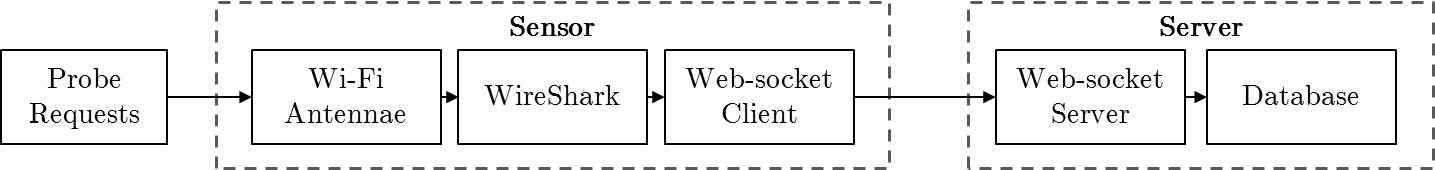
\includegraphics[width=\linewidth]
		{images/datacollection_schematic.jpeg}
	\caption 
		{Schematic diagram showing the process of collecting and storing probe
		requests using the sensor}
	\label{datacollection_schematic} 
\end{figure}

The next step after collecting data was to estimate the footfall or pedestrian
activity from them. We identified the following potential uncertainties which
arise from our collection methodology. 

\begin{enumerate} 
\item 
\textbf{Background noise} - since the extent to which Wi-Fi signals travel
		differs subject to various factors such as interference and humidity, it
		is close to impossible to restrict our data collection to a finite area
		of interest. This can lead to a significant background noise at certain
		locations. E.g. a phone shop or a bus stop located next to the study
		area can increase the number of probe requests received by the sensor.
		It is important to note that this method may not work effectively on
		study locations with complex configurations such as the source of noise
		and the area of study being located at the same distance from the
		sensor. This aspect is explored in detail in the broader case study in
		the following sections.
\item 
\textbf{MAC randomisation} - The mobile devices in recent years have been using
		randomised 'local' MAC addresses for probe requests to protect the users
		from being tracked. This makes it impossible to tell if the probe
		requests are being sent by the same mobile device which is being
		stationed next to the sensor. This along with the previous problem can
		further increase the magnitude of error by several fold.
\item
\textbf{Mobile ownership} - Since the rate of mobile ownership can vary widely
		across geography and demography, we cannot assume that every mobile
		device translates to one pedestrian footfall. In addition to this, there
		is a long term overall increase in mobile ownership which may lead to
		the number of probe requests collected overtime.
\end{enumerate}

We propose the following internal and external validation methods to tackle each
of these uncertainties.

\begin{figure} 
\centering 
\subfigure [Distribution of signal strengths (dBm) showing the filtering of
		background noise] {\resizebox*{0.45\linewidth}{!}
		{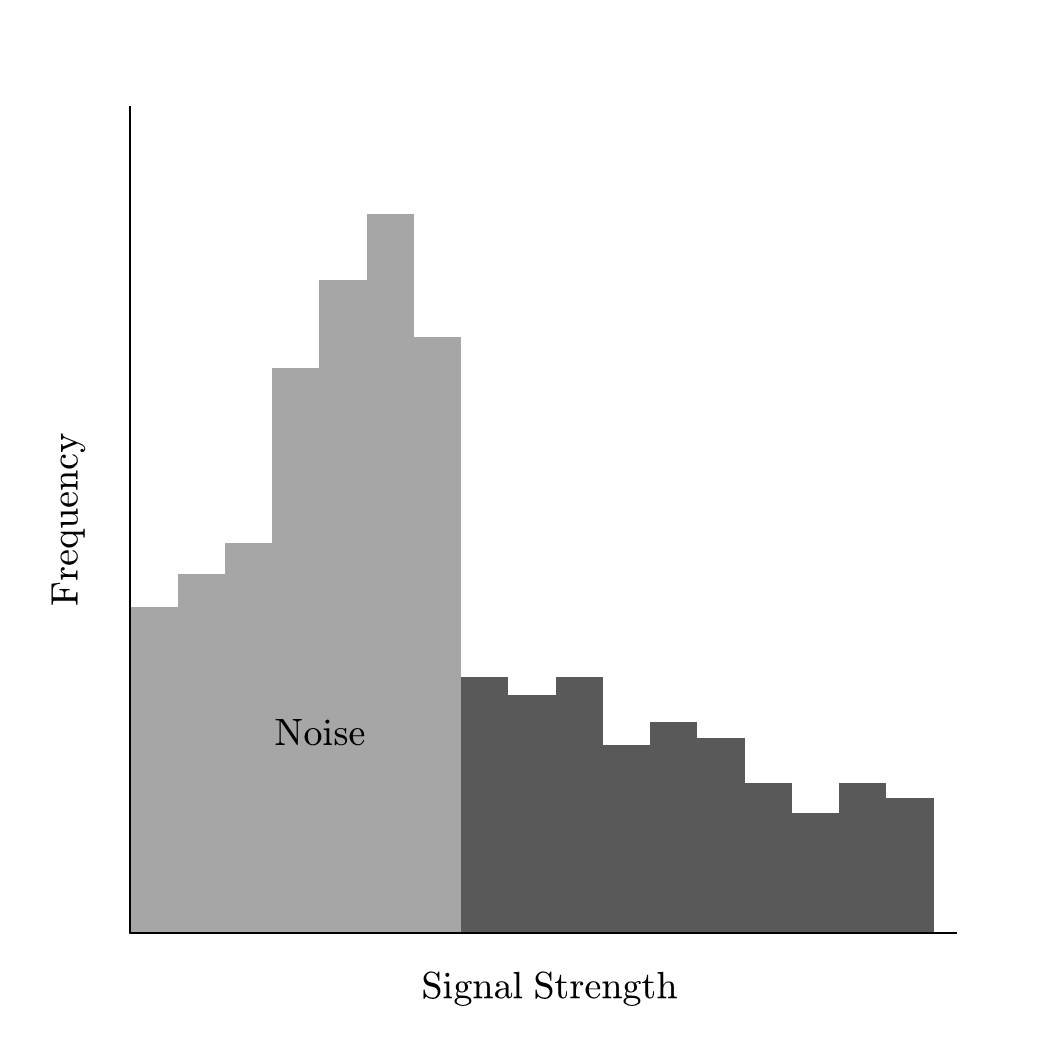
\includegraphics{images/methodology_signalstrength.jpeg}}}
\hspace{20pt}
\subfigure [Clustering probe requests as nodes in a graph using increasing
		sequence numbers] {\resizebox*{0.45\linewidth}{!}
		{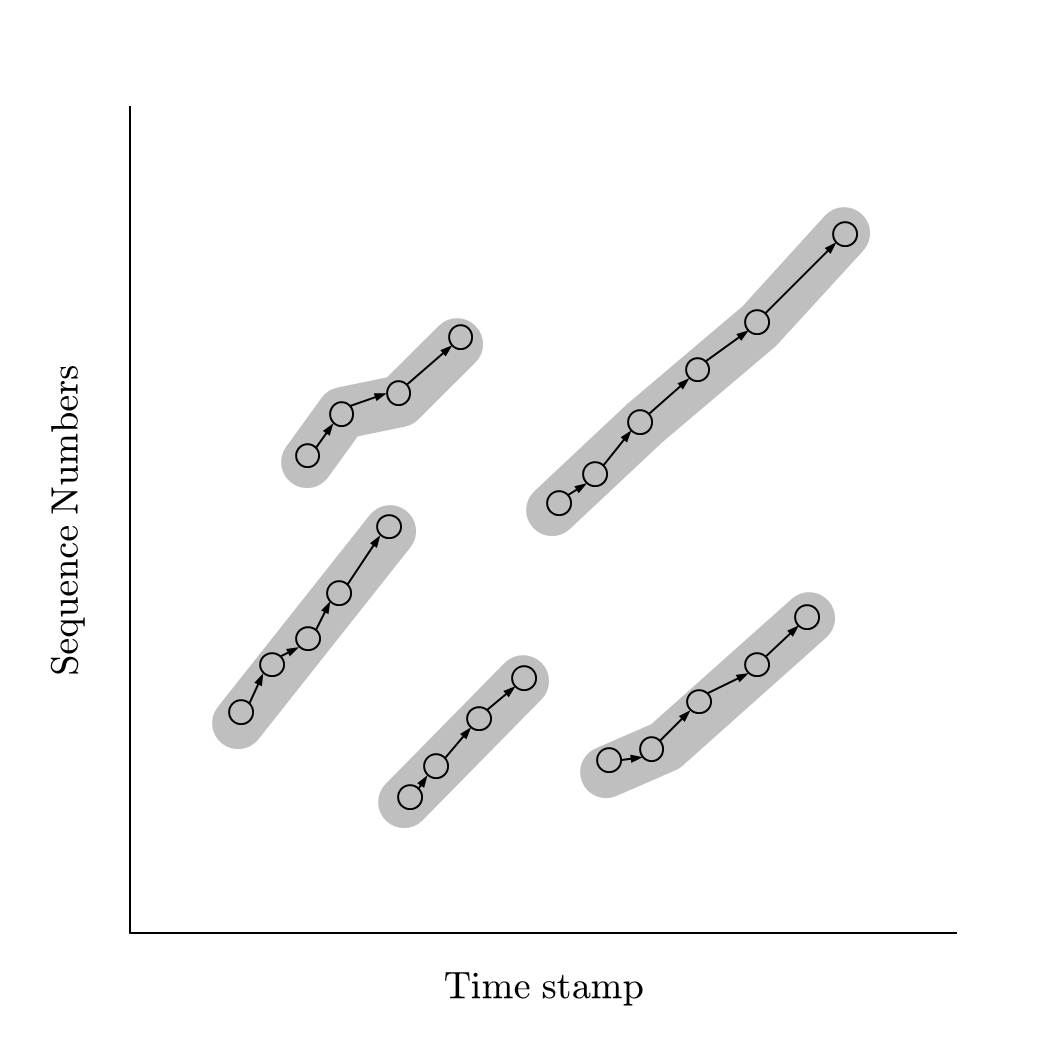
\includegraphics{images/methodology_clustering.jpeg}}}
\caption {Schematic diagrams explaining the methods for filtering by signal
	strength and clustering using sequence numbers}
\label{methodology_schematic}
\end{figure}

\subsection{Filtering with Signal Strength} 

One of the clues that we can use to estimate the distance between the mobile
device and the sensor is the strength of the signal received by the sensor. The
obvious approach here is to try and establish a relationship between the signal
strength and distance first and use this to filter out the unwanted probe
requests. This approach was found not to be feasible since the decay of signal
strength with distance is not always constant. It varies with atmospheric
conditions, presence of obstructions between the source and target, the nature
of these obstructions and the strength (power level) of the source. This
severely limits our ability in establishing a simple conversion between reported
signal strength and distance. There is a need for a method which takes in to
account these variables across various locations.

We assume that in configurations where a specific source of background
noise is at a constant distance, there must be a distinct pattern in the number
of probe requests reporting signal strength corresponding to that distance. For
example, if there is a phone shop next to our sensor where hundreds of phones
regularly send probe requests there should be a sharp rise of number of probe
requests with reported signal strength corresponding to the distance between the
sensor and the phone shop irrespective of the local conditions as shown in
Figure \ref{methodology_schematic}. We could identify these breaks in the data
using traditional one dimensional clustering algorithms such as `jenks natural
breaks', `k-means', `quantile' and `hierarchical clustering', etc. Since we are
only looking for the break in the data and not for absolute values, the
methodology should apply for all the variations due micro site conditions thus
reducing the overall noise in the collected data.

\subsection{Clustering with sequence numbers}

Since our primary unique identifier - MAC address, is being anonymised by new
devices, we need to find other information present in the probe request for use
as a unique identifier. Obvious approach here is to establish a factor of
randomisation and adjust the counts for these probe requests based on this
factor. We found this approach to be not feasible since the proportion of
devices which randomise the MAC addresses increases over time. There is also a
wide variation in the frequency at which the devices randomise the MAC addresses
and the method used for the process. This lead us to look for a more
generalisable approach which is independent of the device model.

From our initial look at the data we found that OUI and the sequence
number of the packet is the most promising information to achieve this.
First we divide our dataset into sets of probe requests with randomised and
non-randomised MAC addresses by looking at the second character of the vendor
part of the MAC address and if it is E, A, 2 or 6, then these addresses are
identified to be randomised. We keep the MAC address as the unique
identifier for the non-randomised requests and further divide the randomised ones in to
sub categories based on their OUI. We then  
identify unique mobile devices from within these sets and assign a unique identifier to each device.

The proposed algorithm creates a graph where the probe requests represented the
nodes, and links are created between them based on the following rules:

\begin{itemize} 
\item A link could go only forward in time. 
\item A link could go from low to high sequence numbers. 
\item A link could exist between nodes with a maximum time difference of
	$\alpha$ - time threshold. 
\item A link could exist between nodes with a maximum sequence number
	difference of $\beta$ - sequence threshold.
\item A node could have only one incoming link and one outgoing link, which is
	the shortest of all such possible links in terms of both time and sequence
	number.
\end{itemize}

The nodes were then assigned a unique id based on the unique connected component
they belong to as shown in Figure \ref{methodology_schematic}. This unique
identifier is used in the place of MAC address for aggregation for the
anonymised probe requests. Though the recycling of sequence number after 4096
leads to multiple unique ids being reported from a single device from a sample
experiment done on randomised probe requests sent by "Google" devices we found
that the sequence number is reset for around 0.05\% of them. We hence assume
this to be inconsequential. 

\subsection{Calibrating with Ground Truth} 

Since mobile device ownership is an external uncertainty to our study and could
arise from variety of spatio - temporal and demographic factors, we propose to
solve this using a sample count done manually at each location.  We can then
calculate an  adjustment factor or an offset for each location by comparing the
sensor based counts and ground truth and in turn it can be used to adjust the
data reliably to reflect the ground truth in absolute numbers for the future.
This calibration can be carried out periodically at these locations to improve
the quality of the estimation.
